\documentclass[a4,center,fleqn]{NAR}

% Enter dates of publication
\copyrightyear{2017}
\pubdate{XX September XXXX}
\pubyear{XXXX}
\jvolume{XX}
\jissue{XX}

%\articlesubtype{This is the article type (optional)}
% \usepackage{xr-hyper}
% \externaldocument[ ]{riboSeed_NAR_suppl}

\usepackage{caption}
\graphicspath{ {../riboSeed/Waters_et_al_2017/ms/riboFigs/} }  %  set the path to the figures

\begin{document}

\title{riboSeed: leveraging prokaryotic genomic architecture to assemble across ribosomal regions}

\author{%
  Nicholas R. Waters\,$^{1,2}$
  Florence Abram\,$^{1}$
  Fiona Brennan\,$^{1,3}$
  Ashleigh Holmes\,$^{4}$
  and Leighton Pritchard$^{2}$
  \footnote{To whom correspondence should be addressed.
      Tel: +44 (0) 1382 568827; E-mail: leighton.pritchard@hutton.ac.uk
  }
}
\address{
  $^{1}$Department of Microbiology, School of Natural Sciences, National University of Ireland, Galway, Ireland \\
  $^{2}$Information and Computational Sciences, James Hutton Institute, Invergowrie, Dundee DD2 5DA, Scotland\\
  $^{3}$Soil and Environmental Microbiology, Environmental Research Centre, Teagasc, Johnstown Castle, Wexford, Ireland\\
  $^{4}$Cell and Molecular Sciences, James Hutton Institute, Invergowrie, Dundee DD2 5DA, Scotland\\
}
% $^{1}$Affiliation of Corresponding Author
% and
% $^{2}$Affiliation of Both Co-Authors}
% Affiliation must include:
% Department name, institution name, full road and district address,
% state, Zip or postal code, country

\history{%
Received January 1, 2009;
Revised February 1, 2009;
Accepted March 1, 2009}

\maketitle

\begin{abstract}
The vast majority of bacterial genome sequencing has been performed using Illumina short reads. Because of the inherent difficulty of resolving repeated regions with short reads alone, only \textasciitilde10\% of sequencing projects have resulted in a closed genome. The most common repeated regions are those coding for ribosomal operons (rDNAs), which occur in a bacterial genome between 1 and 15 times, and are typically used as sequence markers to classify and identify bacteria. Here, we exploit conservation of the genomic context in which rDNAs occur across taxa to improve assembly of these regions relative to \textit{de novo} sequencing by using the conserved nature of rDNAs across taxa and the uniqueness of their flanking regions within a genome. We describe a method which constructs targeted pseudocontigs generated by iteratively assembling reads that map to a reference genome's rDNAs. These pseudocontigs are then used to more accurately assemble the newly-sequenced chromosome. We show that this method, implemented as riboSeed, correctly bridges across adjacent contigs in bacterial genome assembly and, when used in conjunction with other genome polishing tools, can result in closure of a genome.
\end{abstract}

\section{Introduction}
\begin{figure}[!th]
  \centering
  \begin{center}
  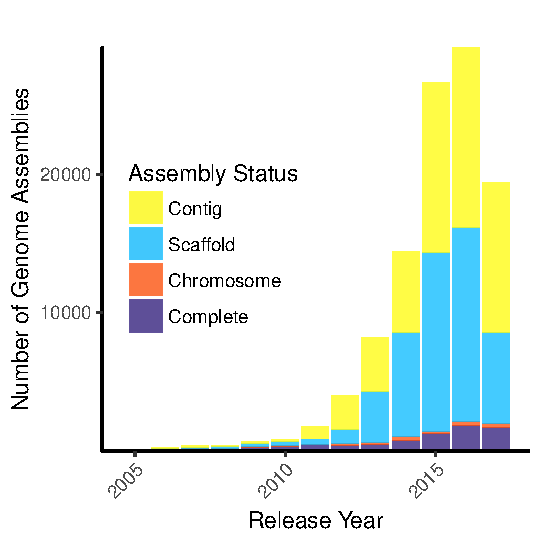
\includegraphics[width=.85\columnwidth]{2017-09-14_plot1}
  \end{center}
  \caption{Counts of bacterial assemblies in NCBI Genome database according to completion level by release year; the four levels (Complete, Chromosome, Scaffold, and Contig) are ordered from complete to most fragmented.  Note that Illumina HiSeq was released in 2010.  Accessed September 14\textsuperscript{th}, 2017.}
  \label{fig:completions}
  % \begin{tabular}{lrrrrr}
  %   \toprule
  %   Date & Total & Complete & Chromosome & Scaffold & Contig \\
  %   \colrule
  %   January 4\textsuperscript{th}, 2017 & 85799 & 6255 & 1143 & 39972 & 38429  \\
  %   May 17\textsuperscript{th}, 2017 & 96849 & 7212 & 1254 & 42839 & 43899\\
  %   \botrule
  %   \multicolumn{3}{l}{
  %   \tiny Source: \url{https://www.ncbi.nlm.nih.gov/genome/browse/}}
  % \end{tabular}
\end{figure}
Sequencing bacterial genomes has become much more cost effective and convenient, but the number of complete, closed bacterial genomes remains a small fraction of the total number sequenced (Figure \ref{fig:completions}). Even with the advent of new technologies for long-read sequencing and improvements to short read platforms, assemblies typically remain in draft status due to the computational bottleneck of genome closure\cite{Nagarajan2010,Brouwer2016}. Although draft genomes are often of very high quality and suited for many types of analysis, researchers must choose between working with these draft genomes (and the inherent potential loss of data), or spending time and resources polishing the genome with some combination of \textit{in silico} tools, PCR, optical mapping, re-sequencing, or hybrid sequencing\cite{Nagarajan2010,Utturkar2014}. Many \textit{in silico} genome finishing tools are available, and we summarise several of these in Table \ref{table:tools}.

% **************************************************************
% Keep this command to avoid text of first page running into the
% first page footnotes
\enlargethispage{-65.1pt}
% **************************************************************


\begin{table*}[t]
\centering
\caption{Some of the available \textit{in silico} genome polishing tools for gap closure}
\label{table:tools}
% \resizebox{\textwidth}{!}{
\begin{tabular*}{\textwidth}{p{2.7cm}p{13cm}}
  \toprule
  Tool &  Method Summary \\
  \colrule
  GapFiller\cite{Boetzer2012} & iteratively uses paired-end reads to close contig junctions \\

  GapCloser\cite{Luo2012} & uses paired-end reads to close contig junctions \\

  IMAGE \cite{Tsai2010} & iteratively uses local assemblies of reads belonging to  assembly gaps \\

  CloG \cite{Yang2011} & uses trimmed \textit{de novo} contigs in hybrid assembly followed by a stitching algorithm \\

  FGap \cite{Piro2014,Guizelini2016} & uses BLAST to find potential gap closures from alternate assemblies, libraries or references. \\

  GFinisher \cite{Guizelini2016} & uses GC-skew to refine assemblies \\

  GapFiller \cite{Nadalin2012} &  produces ``long-reads'' from paired-end sequencing data using a local assembler, which can then be used in a \textit{de novo} assembly. \\

  CONTIGuator\cite{Galardini2011} & uses contigs from a \textit{de novo} assembly along with one or more reference sequences to generate a contig map and PCR primer sets to validate in the lab. \\

  Konnector\cite{Vandervalk2015} & uses paired-end reads to make long reads to be used in a Bloom filter representation of a de Bruijn graph \\

  MapRepeat\cite{Mariano2015} & uses a directed scaffolding method to fill in rDNA gaps, but limited to Ion Torrent reads, and affected by inversions between rDNAs \cite{Mariano2016} \\

  GRabB\cite{Brankovics2016} & selectively assembles tandem rDNAs and mitochondria\\
  \botrule
\end{tabular*}
\end{table*}

The Illumina entries in NCBI's Sequence Read Archive (SRA) \cite{Kodama2012a} outnumber all other technologies combined by about an order of magnitude (Table S1). Draft assemblies from these datasets have systematic problems common to short read datasets, including gaps in the scaffolds due to the difficulty of resolving assemblies of repeated regions\cite{Whiteford2005,Treangen2011}. By resolving repeated regions during the assembly process, it may be possible to improve existing assemblies, and therefore obtain additional sequence information from existing short read datasets in the SRA.



The most common repeated regions are those coding for ribosomal RNA operons (rDNAs). As ribosomes are essential for cell function, sequencing of the 16S ribosomal region is widely used to identify prokaryotes and explore microbial community dynamics\cite{Weisburg1991,Clarridge2004,Woese1990,Case2007}. This region is conserved within taxa, yet retains enough variability to act as a bacterial ``fingerprint'' to separate clades informatively. However, the 16S, 23S, and 5S ribosomal subunit coding regions are often present in multiple copies within a single prokaryotic genome, and commonly exhibit polymorphism \cite{Coenye2003,Moreno2002,Lukjancenko2010,Vetrovsky2013}. These long, inexactly repeated regions\cite{Alkan2011} are problematic for short-read genome assembly. As rDNAs are frequently used as a sequence marker for taxonomic classification, resolving their copy number and sequence diversity from short read collections where the assembled genome has collapsed several repeats into a single region could help improve reference databases, increasing the accuracy of community analysis. We present here an \textit{in silico} method, riboSeed, that capitalizes on the genomic conservation of rDNA and flanking sequence within a taxon to improve resolution of these difficult regions and provide a means to benefit from unexploited information in the SRA/ENA short read archives.


riboSeed is most similar in concept to GRabB, the method of Brankovics et al. \cite{Brankovics2016} for assembling mitochondrial and rDNA regions in eukaryotes. Both use targeted assembly, but GRabB does not make inferences about the number of rDNA clusters present in the genome, or take advantage of their genomic context. In riboSeed, genomic context is resolved by exploiting both the rDNA sequences and their flanking regions, harnessing unique characteristics of the broader rDNA region within a single genome to improve assembly.


The riboSeed algorithm proceeds from two observations: first, that although repeated rRNA coding sequences within a single genome are nearly identical, their flanking regions (that is, the neighboring locations within the genome) are distinct in that genome, and second, that the genomic contexts of equivalent rDNA sequences are also conserved within a taxonomic grouping. riboSeed uses only reads that map to rDNA regions from a reference genome, and is not affected by chromosomal rearrangements that occur outside the flanking regions immediately adjacent to each rRNA.


Briefly, riboSeed uses rDNA regions from a closely-related organism's genome to help generate rDNA cluster-specific ``pseudocontigs'' derived only from the input short reads, that are seeded into the raw short reads to generate a final assembly. We refer to this process in this work as \textit{de fere novo} (meaning ``starting from almost nothing'') assembly.



\begin{figure*}[t]
  \begin{center}
  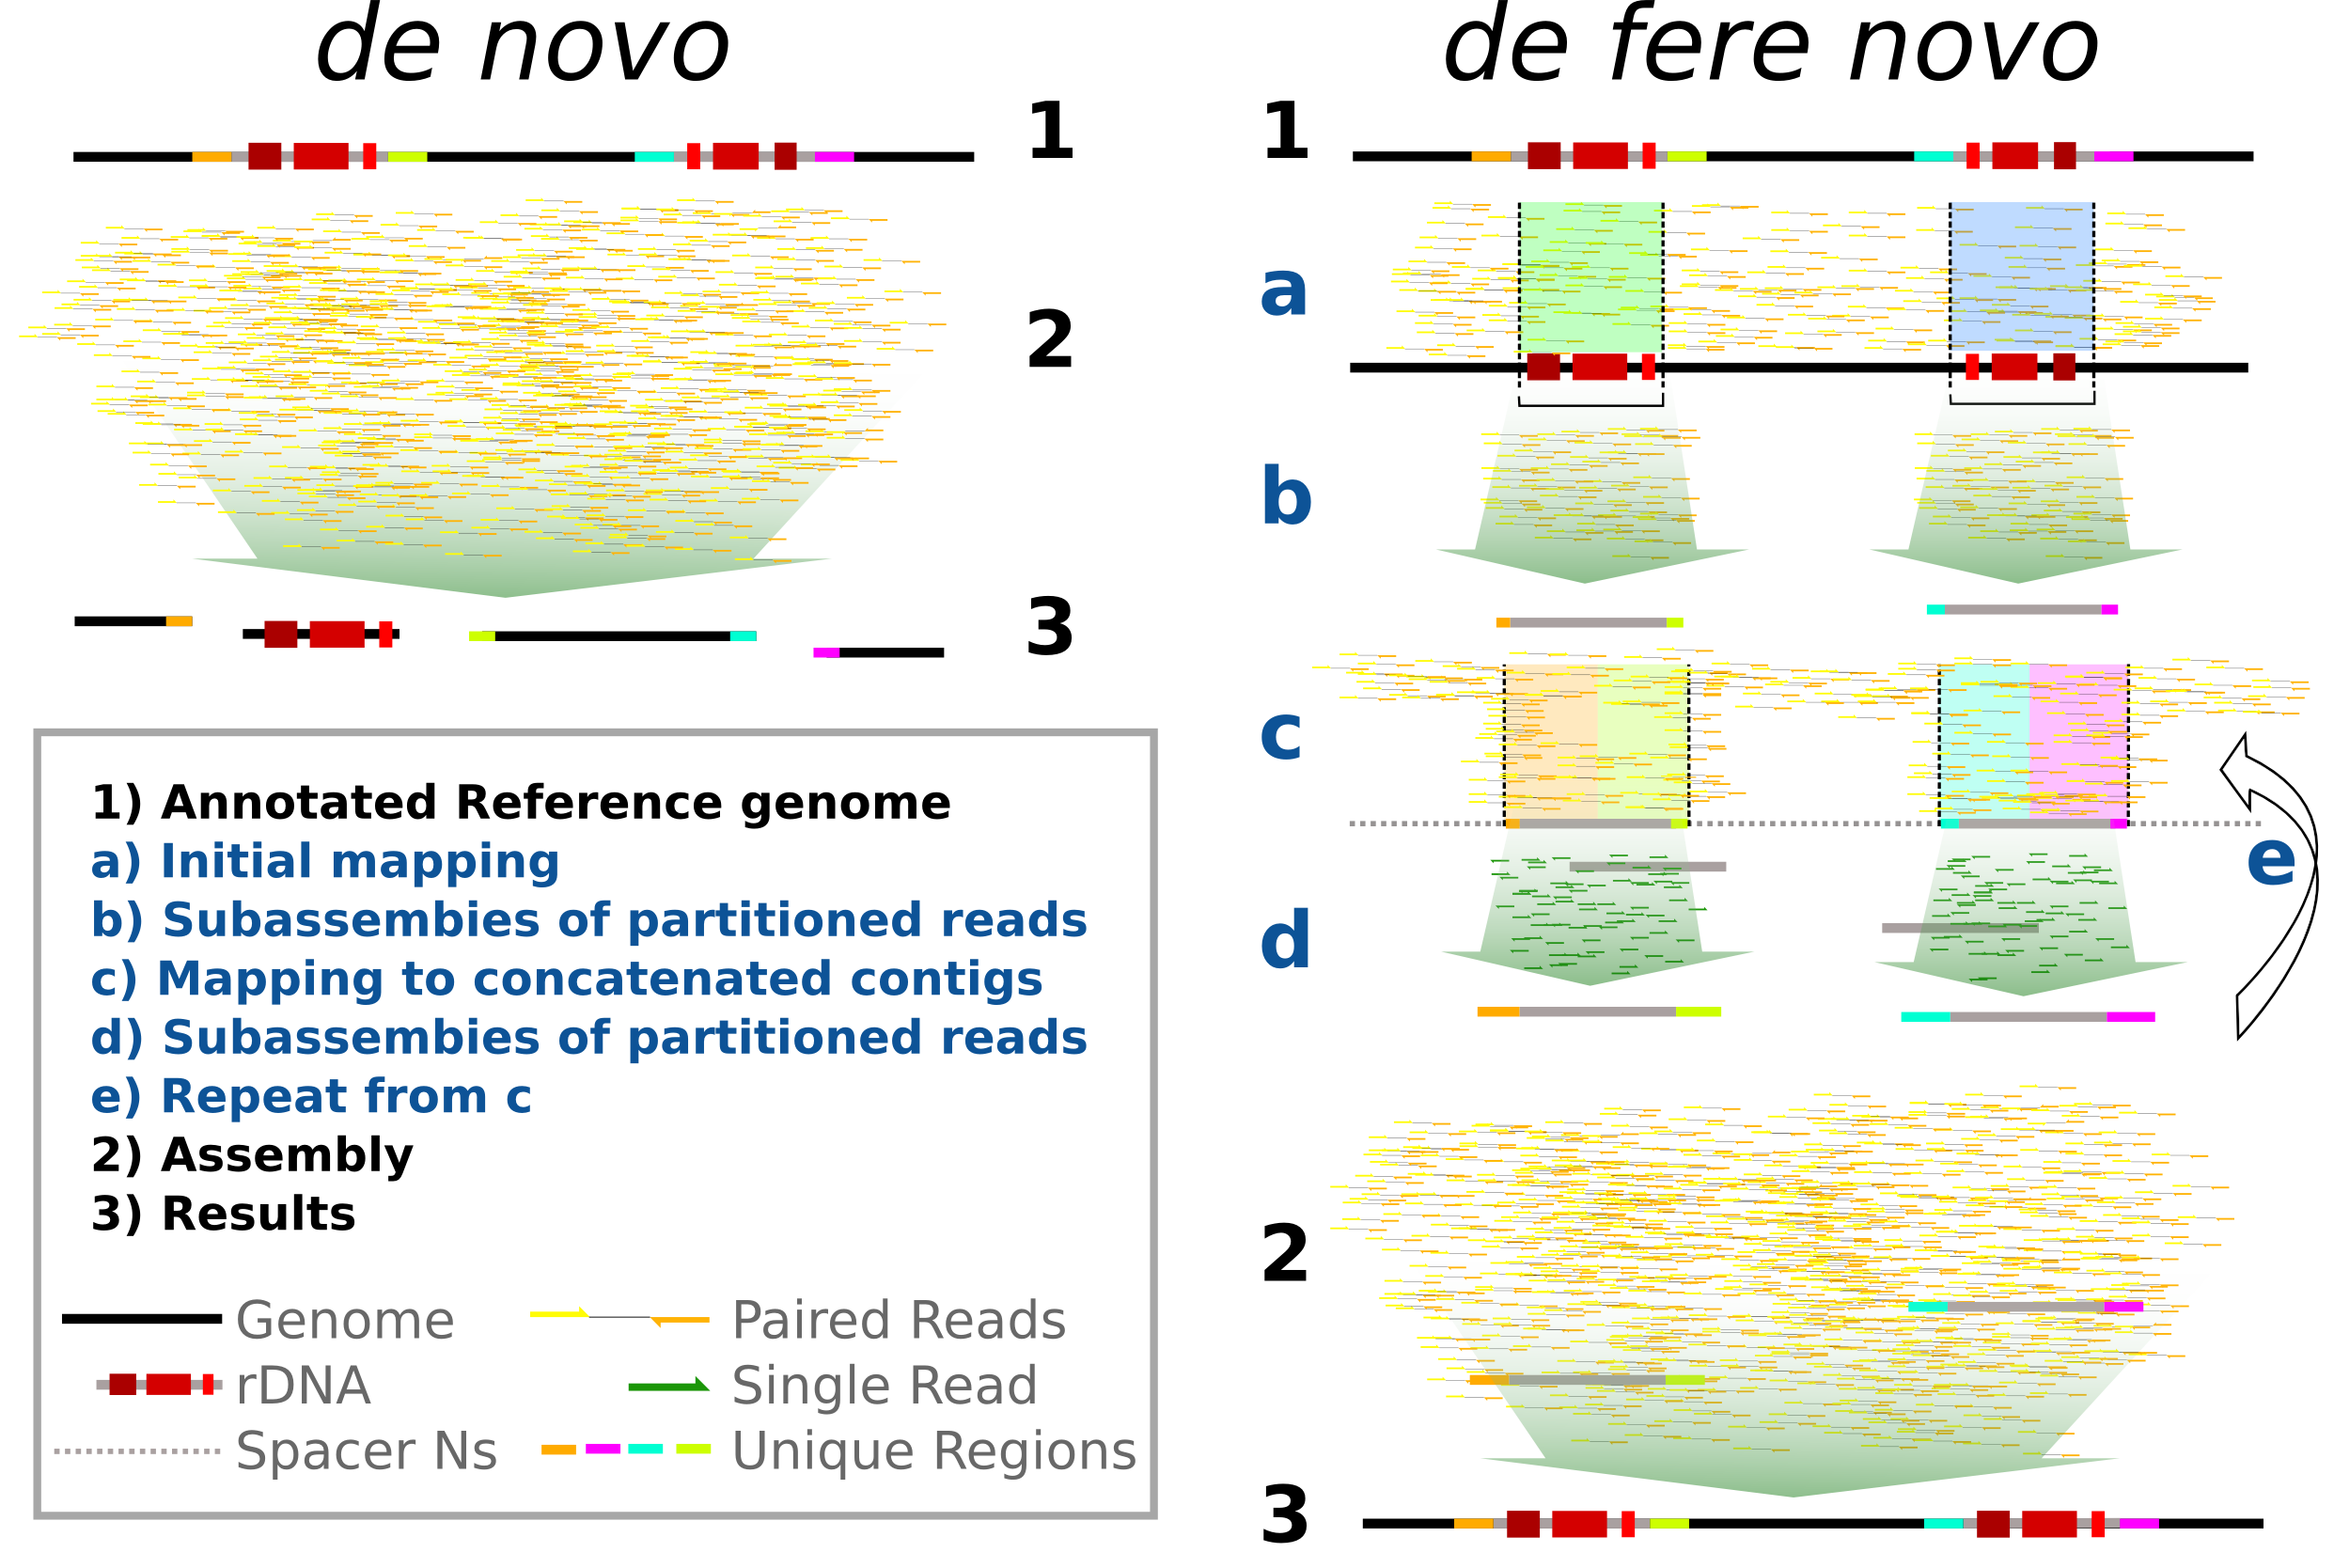
\includegraphics[width=.85\textwidth]{riboSeed_v14}
  \end{center}
  \caption{A comparison of \textit{de novo} assembly to \textit{de fere novo} assembly, as implemented in riboSeed. Reads are mapped to a reference genome, and those reads that align to rDNA and flanking regions are extracted. A subassembly for each group of reads that maps to an rDNA region is constructed to produce a ``pseudocontig'' for each region. These pseudocontigs are concatenated together separated by 1kb of Ns as a spacer. Reads are then iteratively mapped to the concatenated pseudocontigs, extracted, and again subassembled to each region. After the final iteration, the pseudocontigs are included with raw reads in a standard \textit{de novo} assembly. The subassemblies attempt to bridge proper rDNA regions by ensuring that flanking regions (represented here by colors) remain correctly paired. The \textit{de novo} assembly collapses the rDNAs, but \textit{de fere novo} places the rDNAs in the proper genomic context.
  }
  \label{fig:overview}
\end{figure*}


\section{MATERIALS AND METHODS}
We present riboSeed: a software suite that allows users to perform \textit{de fere novo} assembly, given a reference genome sequence from a closely-related organism and single or paired-end short reads to be assembled (Figure \ref{fig:overview}). The code is primarily written in Python3, with accessory shell and R scripts.


riboSeed relies on a closed reference genome assembly that is sufficiently closely-related to the isolate being assembled (which can be estimated using an alignment-free approach such as the KGCAK database\cite{Wang2015b}, or a kmer based method such as Kraken\cite{Wood2014}), in which rDNA regions are assembled and assumed to be in the correct genomic context.

In an ideal scenario, reference selection would consist of two steps:  isolate identification (using Kraken), and then average nucleotide identity analysis to find closest complete reference. We outline protocols for reference selection in Supplementary Information, and in riboSeed documentation at \url{http://riboseed.readthedocs.io/en/latest/REFERENCE.html}.

\subsection*{Usage}
Installation (via either conda, pip, or GitHub), installs the \texttt{ribo} program. Installation using conda also installs third-party tool dependencies, such as SPAdes, and is recommended. The riboseed pipeline can be executed with a single command, \texttt{ribo run}, or under control of the user by means of distinct commands. \texttt{ribo run} performs reannotation of rDNAs in the reference genome (\texttt{scan} command), operon inference (\texttt{select} command), and \textit{de fere novo} assembly (\texttt{seed} command).  The most commonly used parameters are accessible via the \texttt{run} command. Alternatively, the full set of parameters for riboSeed can be defined within a configuration file.

\subsection*{1. Preprocessing}

\textbf{\texttt{scan}}\\
\texttt{scan} uses Barrnap (\url{https://github.com/tseemann/barrnap}) to annotate rRNAs in the reference genome, and EMBOSS's seqret\cite{Rice2000a} to create GenBank, FASTA, and GFF formatted versions of the reference genome. This preprocessing step unifies the annotation vocabulary for downstream processes.\\
\\
\textbf{\texttt{select}}\\
\texttt{select} infers ribosomal operon structure from the genomic location of constituent 16S, 23S and 5S sequences. Jenks Natural Breaks algorithm is then employed to group rRNA annotations into likely operons on the basis of their genomic coordinates, using the number of 16S annotations to set the number of breaks. The output defines individual rDNA clusters and describes their component elements in a plain text file. This output can be manually adjusted before assembly if the clustering does not accurately reflect the known arrangement of operons based on visualization of the annotations in a genome browser.

\subsection*{2. \textit{De Fere Novo} Assembly}

\textbf{\texttt{seed}}\\
\texttt{seed} implements the algorithm described in Figure S1 in the current release. Short reads for the sequenced isolate are mapped to the reference genome using BWA\cite{Li2009}. Reads that map to each annotated rDNA and its flanking regions (where the flanking regions consist of 1kb upstream and 1kb downstream of the rDNA, by default) are extracted into subsets (one subset per cluster). Each subset is independently assembled into a representative pseudocontig with SPAdes\cite{Bankevich2012}, using the reference rDNA regions as a trusted contig (or untrusted, if mapping quality is poor). The resulting pseudocontigs are evaluated for inclusion in future mapping/subassembly iterations based on their length (as discussed below), and concatenated into a pseudogenome, in which pseudocontigs are separated by 1kb of Ns as a spacer. Note that as we are only concerned with the flanking regions, the order in which the pseudocontigs are concatenated is arbitrary; a 1kb spacer length was chosen as an arbitrarily sufficient length to prevent reads from spanning the spacer. This process is repeated in each subsequent iteration, using the previous round's pseudogenome as the reference.


After a specified number of iterations (3 by default), SPAdes is used to assemble all short reads in a hybrid assembly that includes the pseudocontigs from the final iteration as ``trusted contigs'' (or as ``untrusted contigs'' if the mapping quality of reads to that pseudocontig falls below a threshold, defined below). As a control, the short reads are also \textit{de novo} assembled without the pseudocontigs.


Although this implementation of riboSeed uses SPAdes to perform both the subassemblies and the final \textit{de fere novo} assembly, the pseudocontigs could be submitted to any hybrid assembler that accepts short read libraries and contigs. After assembly, the \textit{de fere novo} and \textit{de novo} assemblies are assessed with QUAST\cite{Gurevich2013}.

\begin{figure*}[!t]
  \centering
  \begin{minipage}{.5\textwidth}
  \centering
      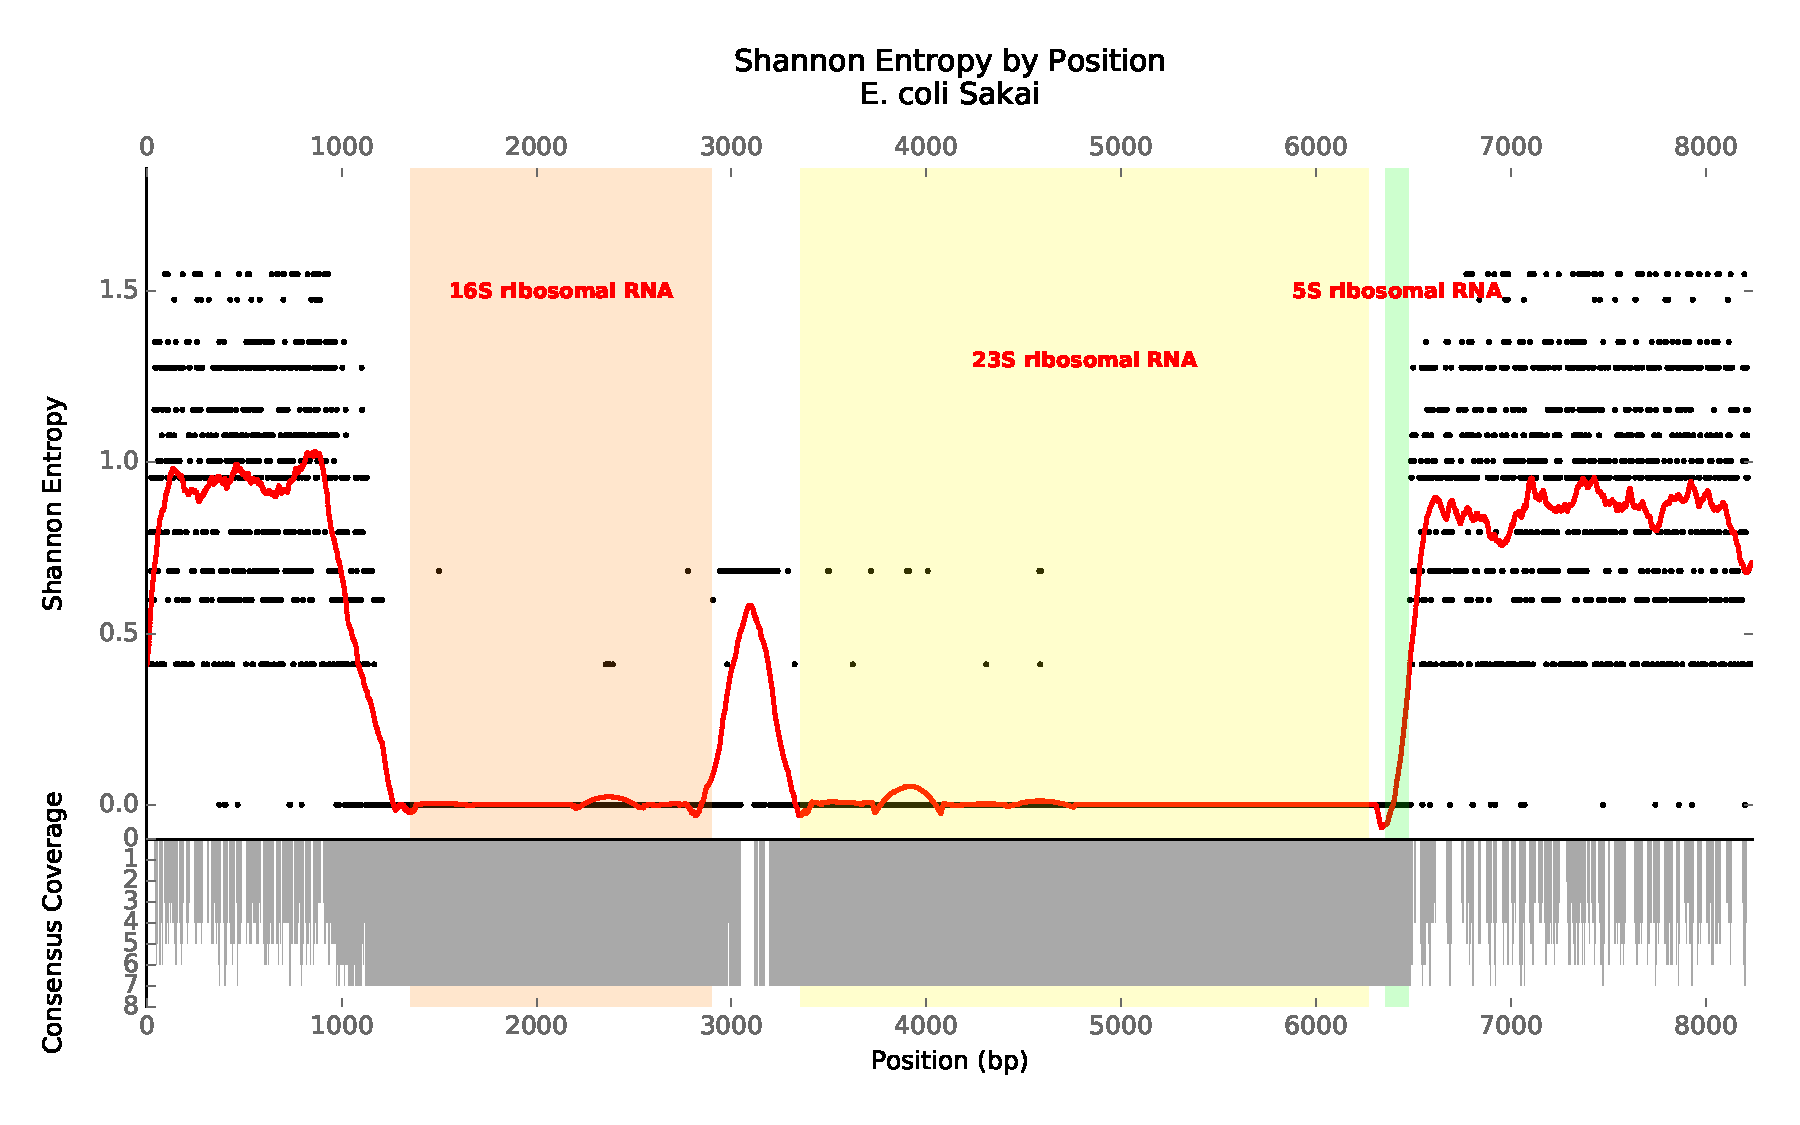
\includegraphics[width=\columnwidth]{entropy_plot}
      {\footnotesize \textbf{a.} All 7 rDNAs from \textit{E. coli} Sakai}
  \end{minipage}%
  \begin{minipage}{.5\textwidth}
  \centering
      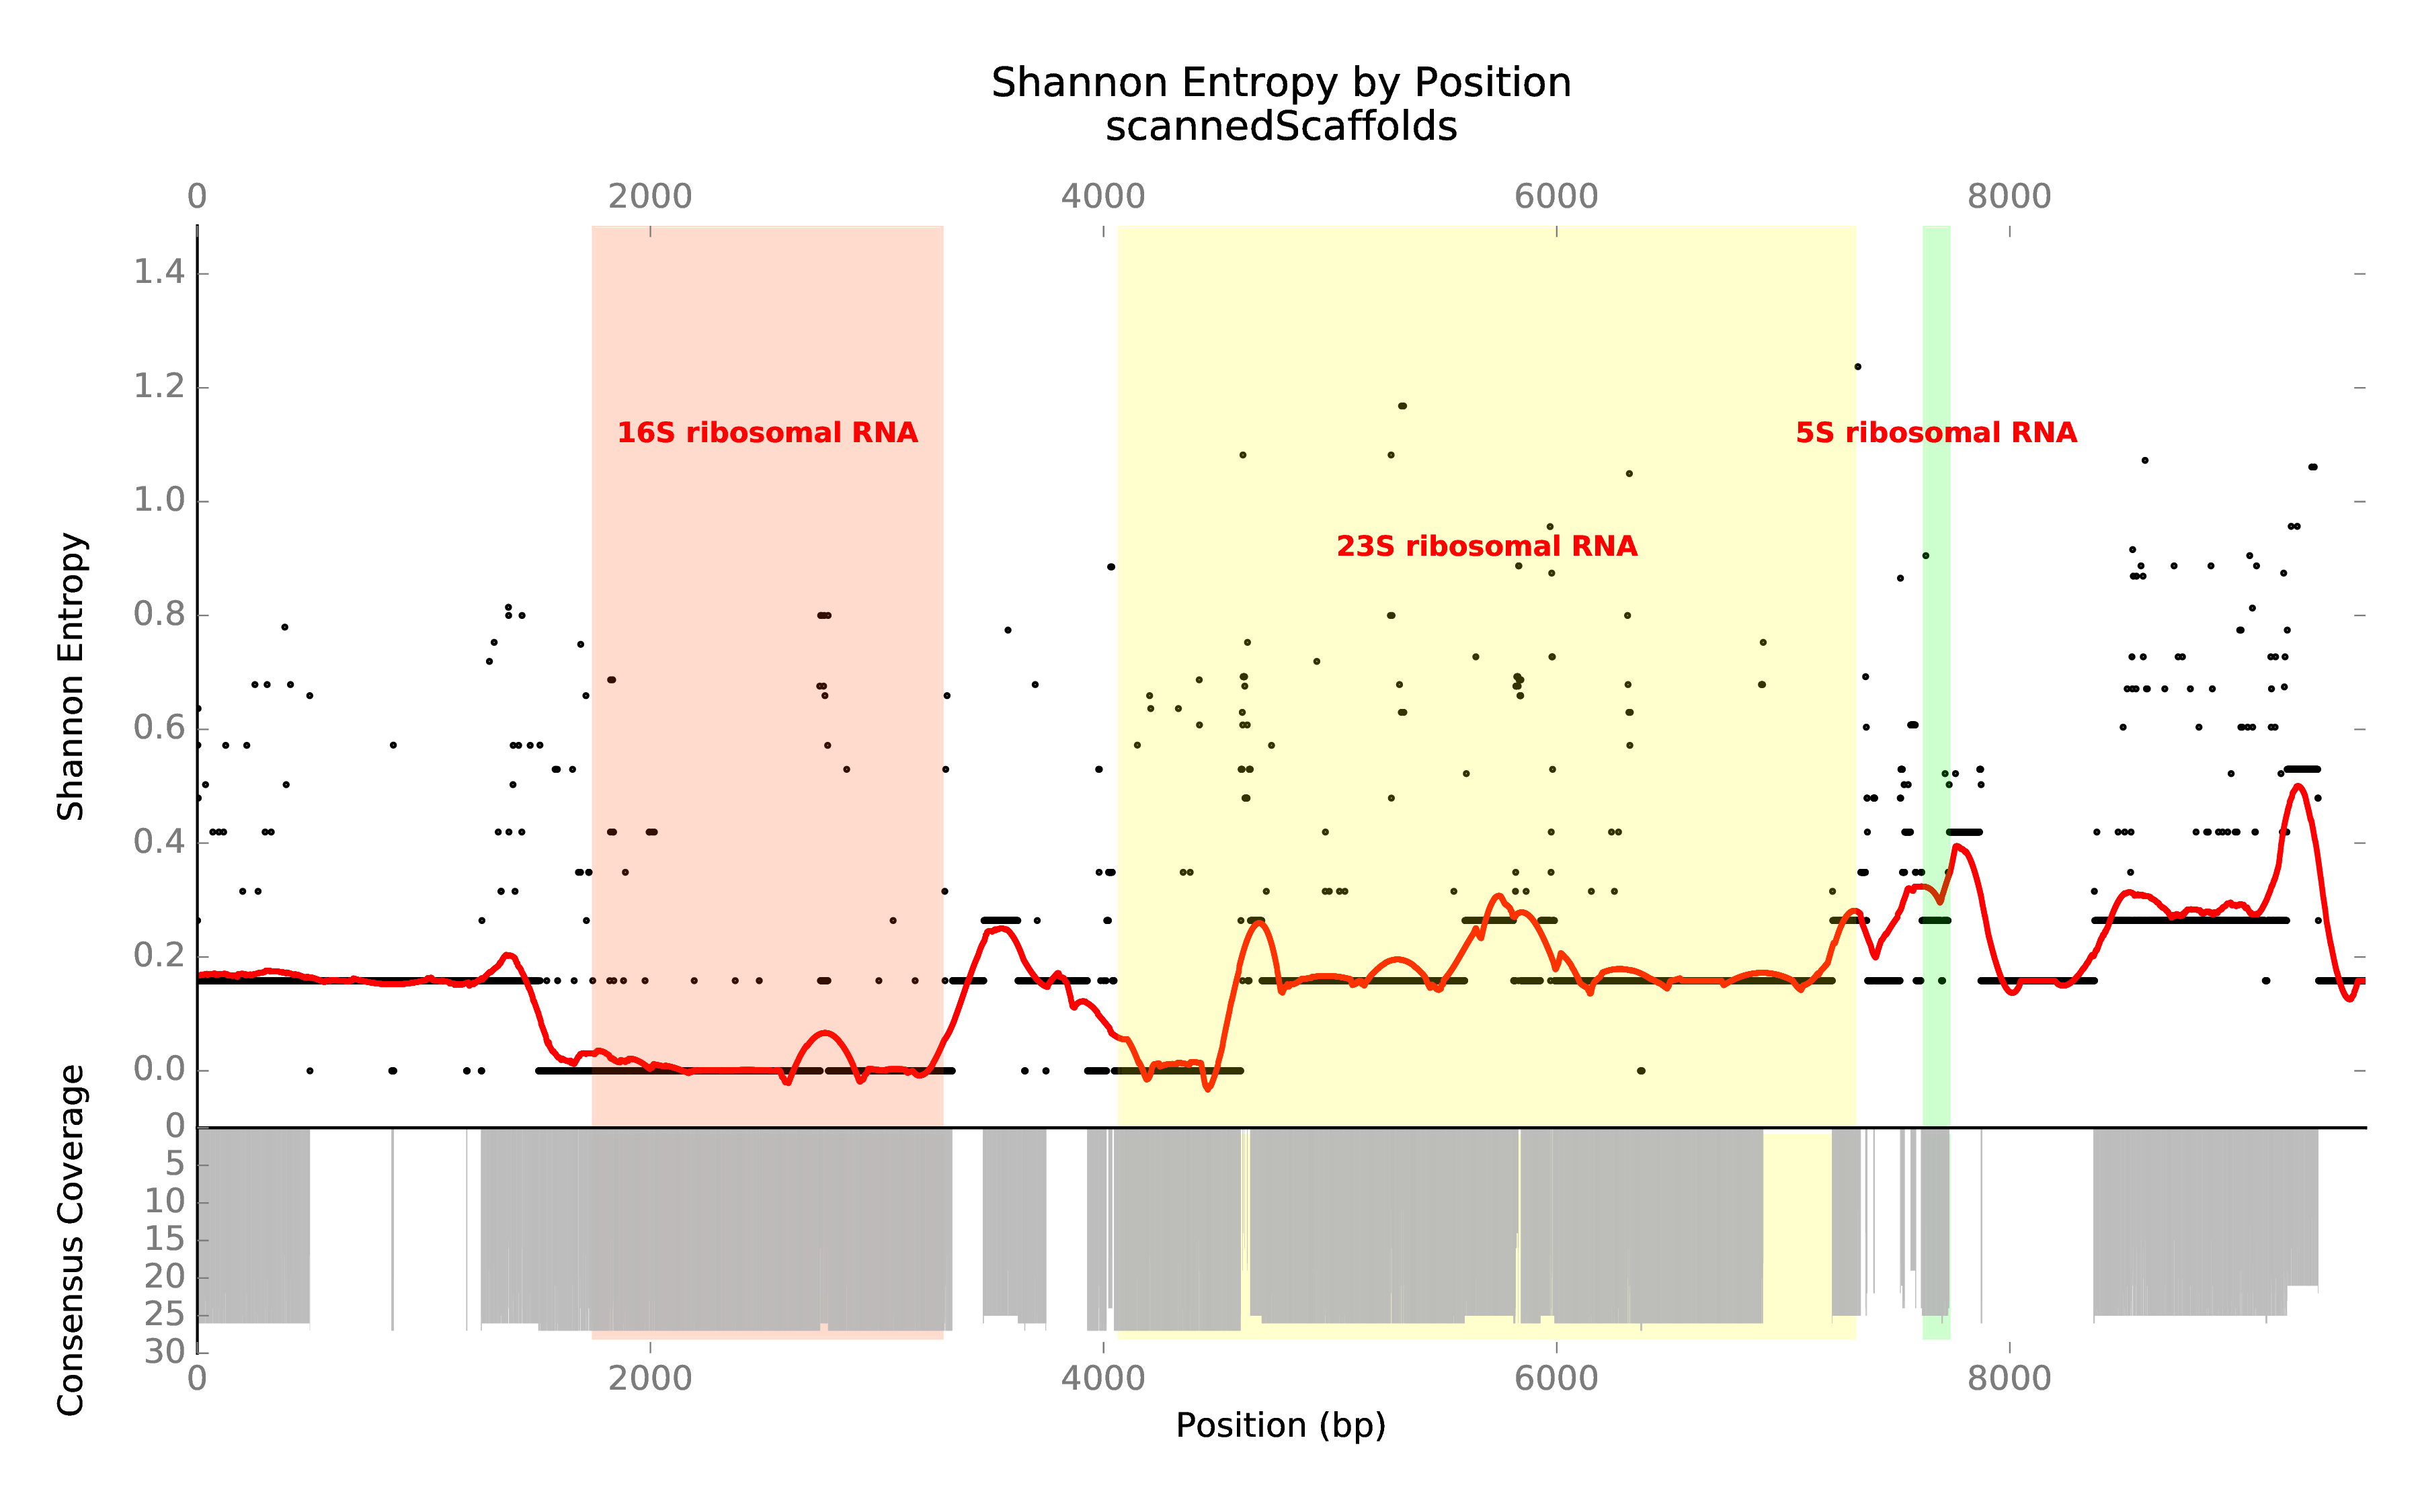
\includegraphics[width=\columnwidth]{entropy_plot_gmbH}
      {\footnotesize\textbf{b.} Homologues of a single rDNA locus from 25 \textit{E. coli} genomes}

  \end{minipage}%

  \caption{
    Consensus coverage depth (gray bars) and Shannon entropy (black points, smoothed with a window size of 351bp as red line) for aligned rDNA regions. For the seven \textit{E. coli} Sakai rDNA regions (a), entropy sharply increases moving away from the the 16S and 5S ends of the operon. In this case flanking regions would be expected to assemble uniquely within a genome. By contrast, the rDNA regions occurring closest to homologous \textit{gmbH} genes from 25 \textit{E. coli} genomes (b) show greater conservation in their flanking regions. This indicates that flanking regions are more conserved for homologous rDNA than for paralogous rDNA operons, and implies that related genomes can be useful reference templates for assembling across these regions. Similar plots for each of the GAGE-B genomes used later for benchmarking can be found in Figure S4.
  }
  \label{fig:entropy}
\end{figure*}

\subsection*{3. Assessment and Visualization}

\textbf{\texttt{score}}\\
\texttt{score} extracts the regions flanking the rDNAs in the reference and in the assemblies generated by riboSeed. The flanking regions from the assembly are matched with the reference flanking regions using BLASTn, and depending on the ordering of the matches, calls junctions as correct, incorrect, or ambiguous joins based on the criteria outlined below.\\
\\
\textbf{\texttt{snag}}\\
\texttt{snag} is provided as a helper tool to produce useful diagnostics and visualisation concerning rDNA sequence in the reference genome. Using the clustering generated by \texttt{select}, sequences for the clusters can be extracted from the genome, aligned, and Shannon entropy \cite{Schmitt1997} plotted with consensus depth for each position in the alignment.\\
\\
\textbf{\texttt{swap}}\\
In addition to \texttt{score}, we recommend assessing the performance of the riboSeed pipeline visually using Mauve\cite{Darling2004,Darling2011}, Gingr\cite{Treangen2014}, or a similar genome assembly visualizer to compare reference, \textit{de novo}, and \textit{de fere novo} assemblies. If contigs appear to be incorrectly joined, the offending \textit{de fere novo} contig can be replaced with syntenic contigs from the \textit{de novo} assembly using the swap script.\\
\\
\textbf{\texttt{stack}}\\
\texttt{stack} uses bedtools\cite{Quinlan2010} and samtools\cite{Li2009} to compare the depths of coverage of reads aligning to the reference genome in the rDNA regions to randomly sampled regions elsewhere in the reference genome. stack takes output from \texttt{scan}, and a BAM file of reads that map to the reference. If the number of \texttt{scan}-annotated rDNAs matches the number of rDNAs in the sequenced isolate, the coverage depths within the rDNAs will be similar to the coverage in other locations in the genome. If the coverage of rDNA regions sufficiently exceeds the average coverage elsewhere in the genome, this may indicate that the reference strain has fewer rDNAs than the sequenced isolate. In this case, using an alternative reference genome may produce improved results.

\subsection*{Availability of data and materials}
The riboSeed pipeline and the datasets generated during the current study are available in the riboSeed GitHub repository, \url{https://github.com/nickp60/riboSeed}. The software is released under the MIT licence.  The modified BugBuilder pipeline can be found at \url{https://github.com/nickp60/BugBuilder}. Reference genomes used for this study can be found in Table S3, and the versions of other software used in this study are found in Table S4.


\section{RESULTS}

Settings used for analyses in this manuscript are the defaults (except where otherwise noted) as of riboSeed version 0.4.35\cite{nicholas_r_waters_2017_832131}. [NOTE: CHANGE TO NEW ZENODO DOI]

\subsection*{Characteristics of rDNA flanking regions}
The use of rDNA flanking sequences to uniquely identify and place rDNAs in their genomic context requires their flanking sequences to be distinct within the genome for each region. This is expected to be the case for most, if not all, prokaryotic genomes. We determined that using 1kb flanking widths was sufficient to include differentiating sequence (Figure S2). To demonstrate this, rDNA and 1kb flanking regions were extracted from \textit{E. coli} Sakai \cite{Hayashi2001} (BA000007.2), in which the rDNAs have been well characterized\cite{Ohnishi2000}. These regions were aligned with MAFFT\cite{Katoh2002}, and their consensus depth and Shannon entropy calculated for each position in the alignment (Figure \ref{fig:entropy}a).

Figure \ref{fig:entropy}a (and Figure S4) shows that within a single genome the regions flanking rDNAs are variable between operons. This enables unique placement of reads at the edges of rDNA coding sequences in their genomic context (i.e. there is not likely to be confusion between the placements of rDNA edges within a single genome).

In \textit{E. coli} MG1655, the first rDNA is located 363 bases downstream of \textit{gmhB} (locus tag b0200). Homologous rDNA regions were extracted from 25 randomly selected complete \textit{E. coli} chromosomes (Table S2).  We identified the 20kb region surrounding \textit{gmhB} in each of these genomes, then annotated and extracted the corresponding rDNA and flanking sequences. These sequences were aligned with MAFFT, and the Shannon entropies and consensus depth plotted (Figure \ref{fig:entropy}b).

Figure \ref{fig:entropy}b shows that equivalent \textit{E. coli} rDNAs, plus their flanking regions, are well-conserved across several related genomes. Assuming that individual rDNAs are monophyletic within a taxonomic group, short reads that can be uniquely placed on a related genome's rDNA as a reference template are also likely able to be uniquely-placed in the appropriate homologous rDNA of the genome to be assembled.

Taken together, when these two properties hold, this allows for unique placement of reads from homologous rDNA regions in the appropriate genomic context. These ``anchor points'' effectively reduce the number of branching possibilities in de Bruijn graph assembly for each individual rDNA, and thereby permit a complete balanced path through the full rDNA region.

\subsection*{Validating assembly across rDNA regions}

To evaluate the performance of \textit{de fere novo} assembly compared to \textit{de novo} assembly methods, we used Mauve to visualize syntenic regions and contig breaks of each assembly in relation to the reference genome that was used to generate pseudocontigs. We categorized each rDNA in an assembly as either correct, unassembled, or incorrect, as follows.

An rDNA assembly was classed as ``correct'' if two criteria were met: (i) the assembly merged two contigs across a rDNA region such that, based on the reference, the flanking regions of the \textit{de fere novo} assembly were syntenous with those of the reference; and (ii) the assembled contig extends at least 90\% of the flanking length. An assembled cluster was defined as ``unassembled'' if the ends of one or more contigs aligned within the rDNA or flanking regions (signalling that extension across the rDNA region was not achieved). Finally, if two contigs assembled across a rDNA region in a manner that conflicted with the orientation indicated in the reference genome, suggesting missasembly, the rDNA region was deemed as ``incorrect''.

In all cases, SPAdes was used with the same parameters for both \textit{de fere novo} assembly and \textit{de novo} assembly, apart from the addition of pseudocontigs in the \textit{de fere novo} assembly.

\subsection*{Simulated reads with artificial genome}


\begin{figure}[!b]
    \centering
    \hspace*{-.7cm}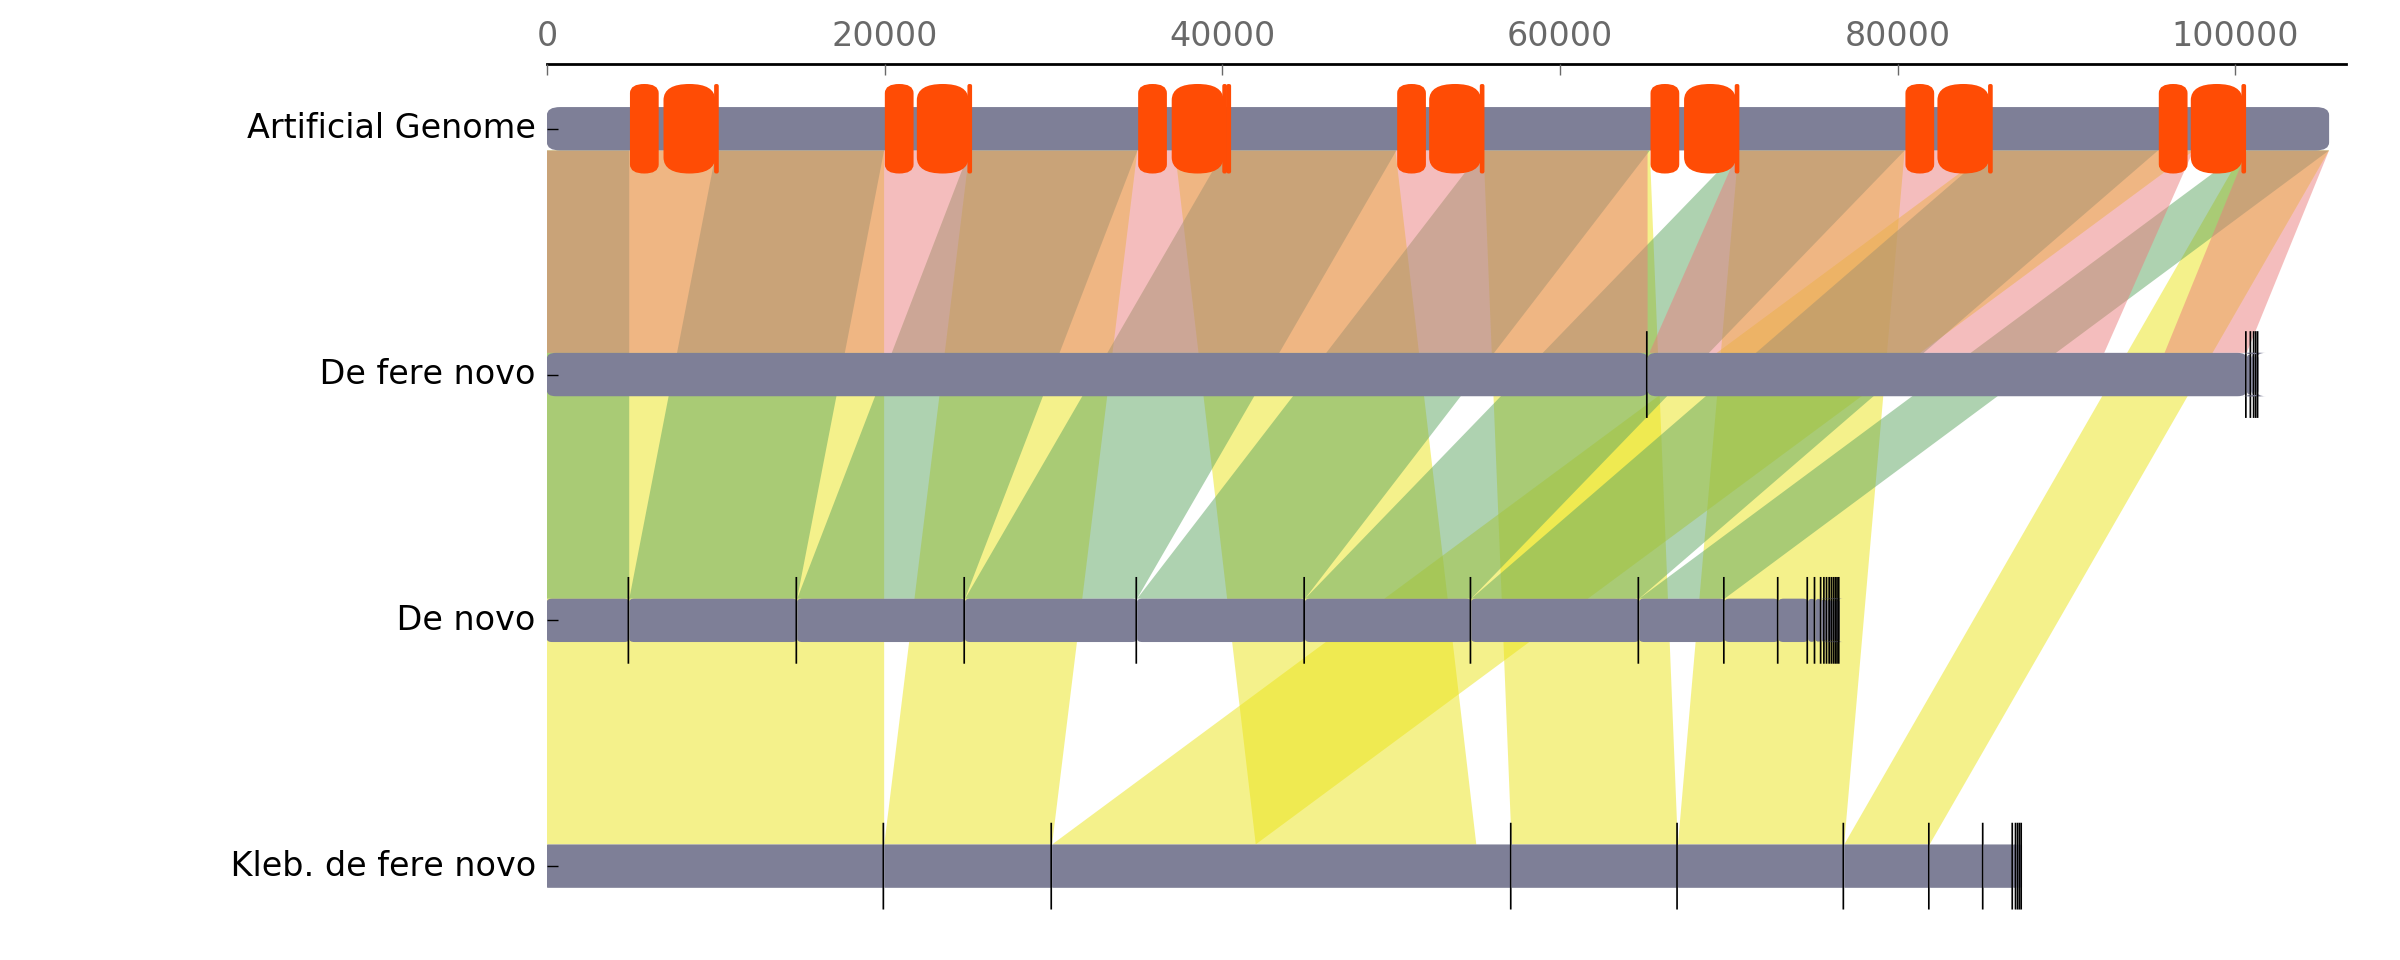
\includegraphics[width=1.2\columnwidth]{PrettyMauve}
    \caption{Representative Mauve output describing the results of riboSeed assemblies of simulated reads generated by pIRS from the concatenated \textit{E. coli} Sakai artificial genome. From top to bottom: artificial reference chromosome; rDNA clusters (red bars); \textit{de fere novo} assembly (\textit{E. coli} reference), \textit{de novo} assembly (\textit{E. coli} reference), and \textit{de fere novo} assembly (\textit{K. pneumoniae} reference). riboSeed with \textit{E. coli} reference assembles 4 of 7 rDNA regions, but the \textit{de novo} assembly recovers no rDNA regions correctly.
}
\label{fig:artificial}
\end{figure}


To create a small dataset for testing, we extracted all 7 distinct rDNA regions from the \textit{E. coli} Sakai genome (BA000007.2), including 5kb upstream and downstream flanking sequence, using the tools \texttt{scan}, \texttt{select} and \texttt{snag}. Those regions were concatenated to produce a \textasciitilde100kb artificial test chromosome (see supplementary methods). pIRS\cite{Hu2012} was used to generate simulated reads (100bp, 300bp inserts, stdev 10, 30-fold coverage, built-in error profile) from this test chromosome. These reads were assembled using riboSeed, using the \textit{E. coli} MG1655 genome (NC\_000913.3) as a reference.  Simulation was repeated 8 times to assess variability of method performance on alternative read sets generated from the same source sequence.


The \textit{de fere novo} assembly bridged 4 of the 7 rDNA regions in the artificial genome, while the \textit{de novo} assembly method failed to bridge any (Table S2). To illustrate how the choice of reference sequence determines the ability to assemble correctly through rDNA regions, we ran riboSeed with the same \textit{E. coli} reads using pseudocontigs derived from the \textit{Klebsiella pneumoniae} HS11286 (CP003200.1) reference genome\cite{Liu2012}. The \textit{de fere novo} assembly with pseudocontigs from \textit{K. pneumoniae} failed, as the reference proved to be too divergent from the reads; this behaviour can be changed by the user, but it acts as a check against applying riboSeed to an inappropriate dataset.


\subsection*{Effect of reference sequence identity on riboSeed performance}
To investigate how riboSeed assembly is affected by choice of reference strain, we implemented a simple mutation model to generate reference sequence variants of the artificial chromosome described above, with a specified rate of mutation. A simple model of geometrically-distributed mutations at a desired mutation frequency applied across all bases uniformly does not address the disparity of conservation between rDNAs and their flanking region, but a second model was also applied wherein substitutions were allowed only within the rDNA flanking regions. We then assembled the artificial genome's reads using the mutated artificial genome as a reference, using these models (Figure \ref{fig:degen}).  Because the range of substitution exceeded our recommended threshold sequence identity, a dropoff is observed at the  substituttion rate of .2 (corresponding to the 80\% mapping percentage threshold).


\begin{figure}[!b]
  \centering
    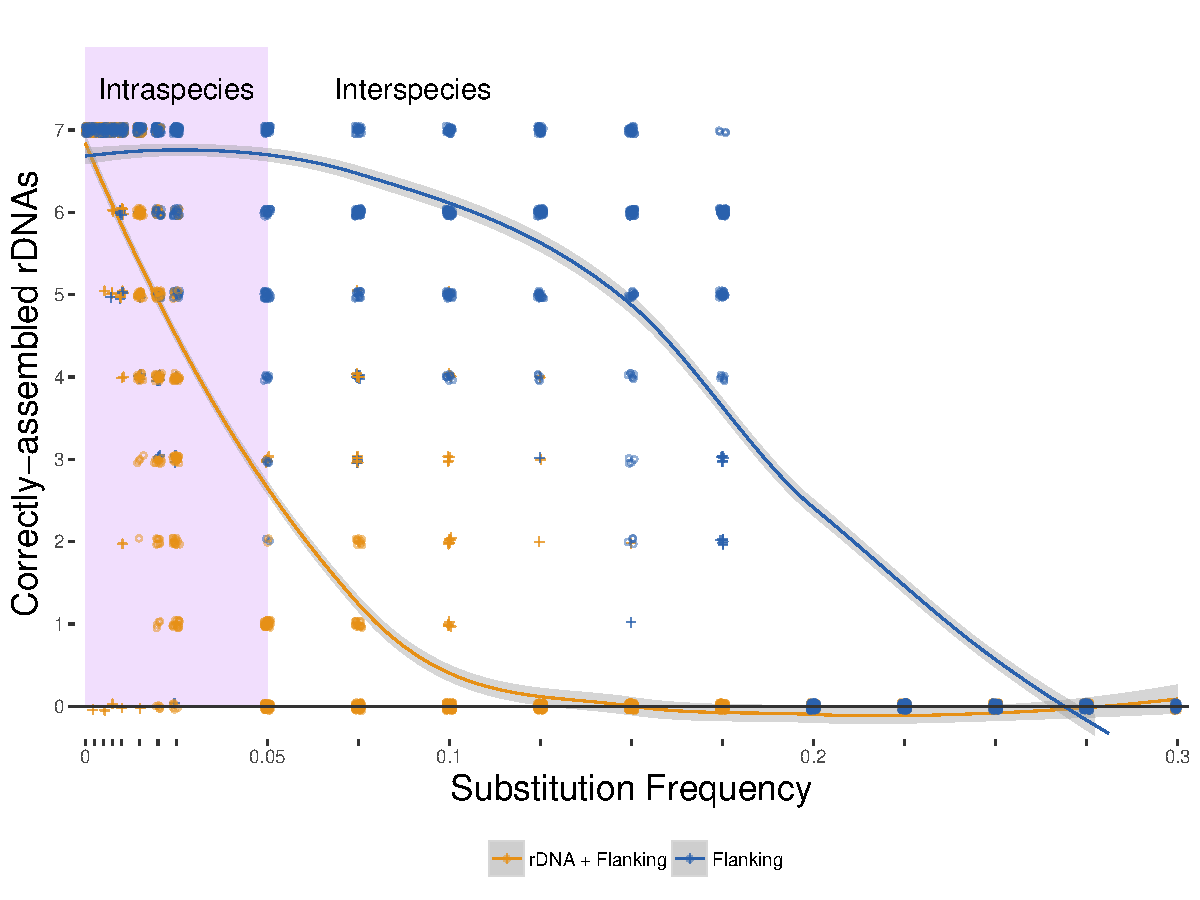
\includegraphics[width=.9\columnwidth]{degenerate_lineplot}
  \caption{Variants of the artificial genome with substitution frequencies between 0 and 0.3 (i.e. up to 300 substitutions per kb). Correctly-assembled rDNAs were counted, and the distribution of results shown against the appropriate substitution frequency. Results are shown for models where substitutions are permitted throughout the chromosome (orange), and only in the flanking regions (blue), the latter approximating the relative rate of substitution in rDNA and flanking regions. Lilac area corresponds to substitution frequencies resulting in average sequence identity over 95\%, denoting a estimated species boundary. Loess smoothing was used for the blue and yellow lines. Outliers are shown as $+$'s. N=100.}
  \label{fig:degen}
\end{figure}


To obtain an estimate of substitution rate for the \textit{E. coli} strains used above, Parsnp\cite{Treangen2014} and Gingr\cite{Treangen2014} were used to identify SNPs in the 25 genomes (Figure \ref{fig:entropy}), with respect to the same region in \textit{E. coli} Sakai. An average substitution rate of 0.0035 was observed. Compared to the results from the simulated genomes, we could expect successful riboSeed performance under the model of mutated flanking regions, and partial success under the model of substitutions throughout the region.


Figure \ref{fig:degen} indicates that the more similar the reference sequence is to the genome being assembled, the greater the likelihood of correctly assembling through rDNA regions. When mutating only the flanking regions (Figure \ref{fig:degen}), which more closely resembles the relative sustitution frequencies of the rDNA regions, the procedure correctly assembles rDNAs with tolerance to substitution frequencies up to approximately 30 substitutions per kb.  With the widely-adopted average nucleotide identity species boundary of 95\% \cite{Goris2007a}, it could be concluded that riboSeed will correctly place and assemble nearly all rDNA regions when using a reference within the same species, and that moderate success can be achieved even when using a more distantly-related reference.



\begin{figure}[!ht]
  \centering
  \begin{minipage}{.45\textwidth}
    \centering
    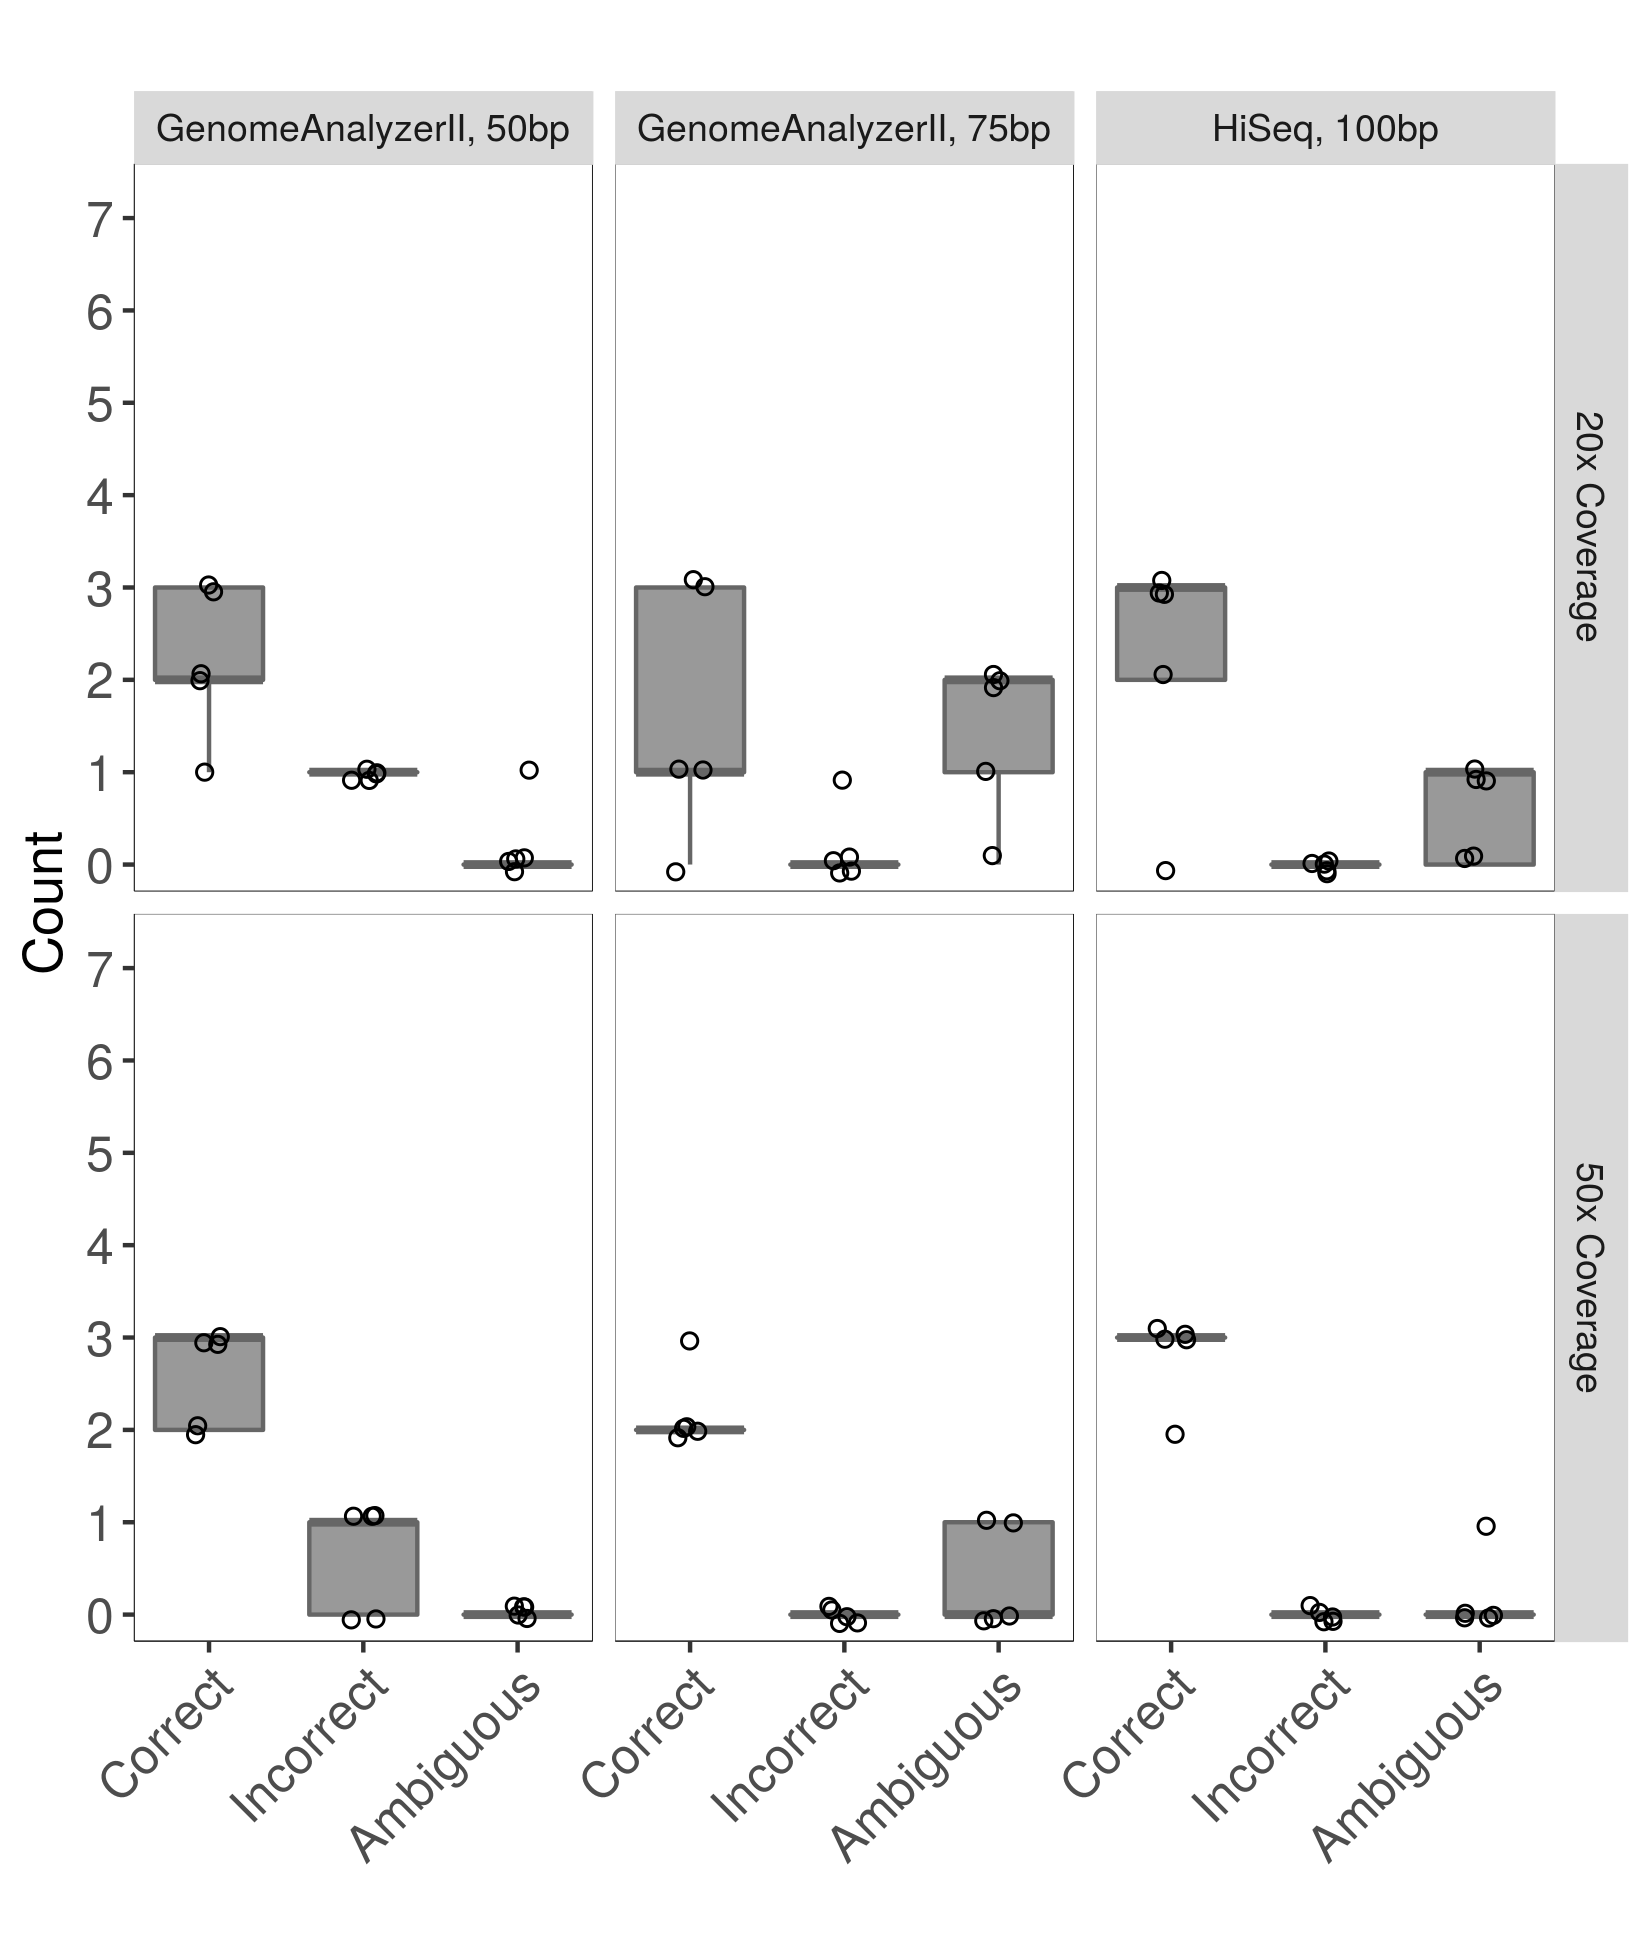
\includegraphics[width=.8\columnwidth]{coli}

    {\footnotesize \textbf{a.} \textit{E. coli} rDNA Assembly}
    \label{fig:sim_coli}
  \end{minipage}

  \begin{minipage}{.45\textwidth}
    \centering
    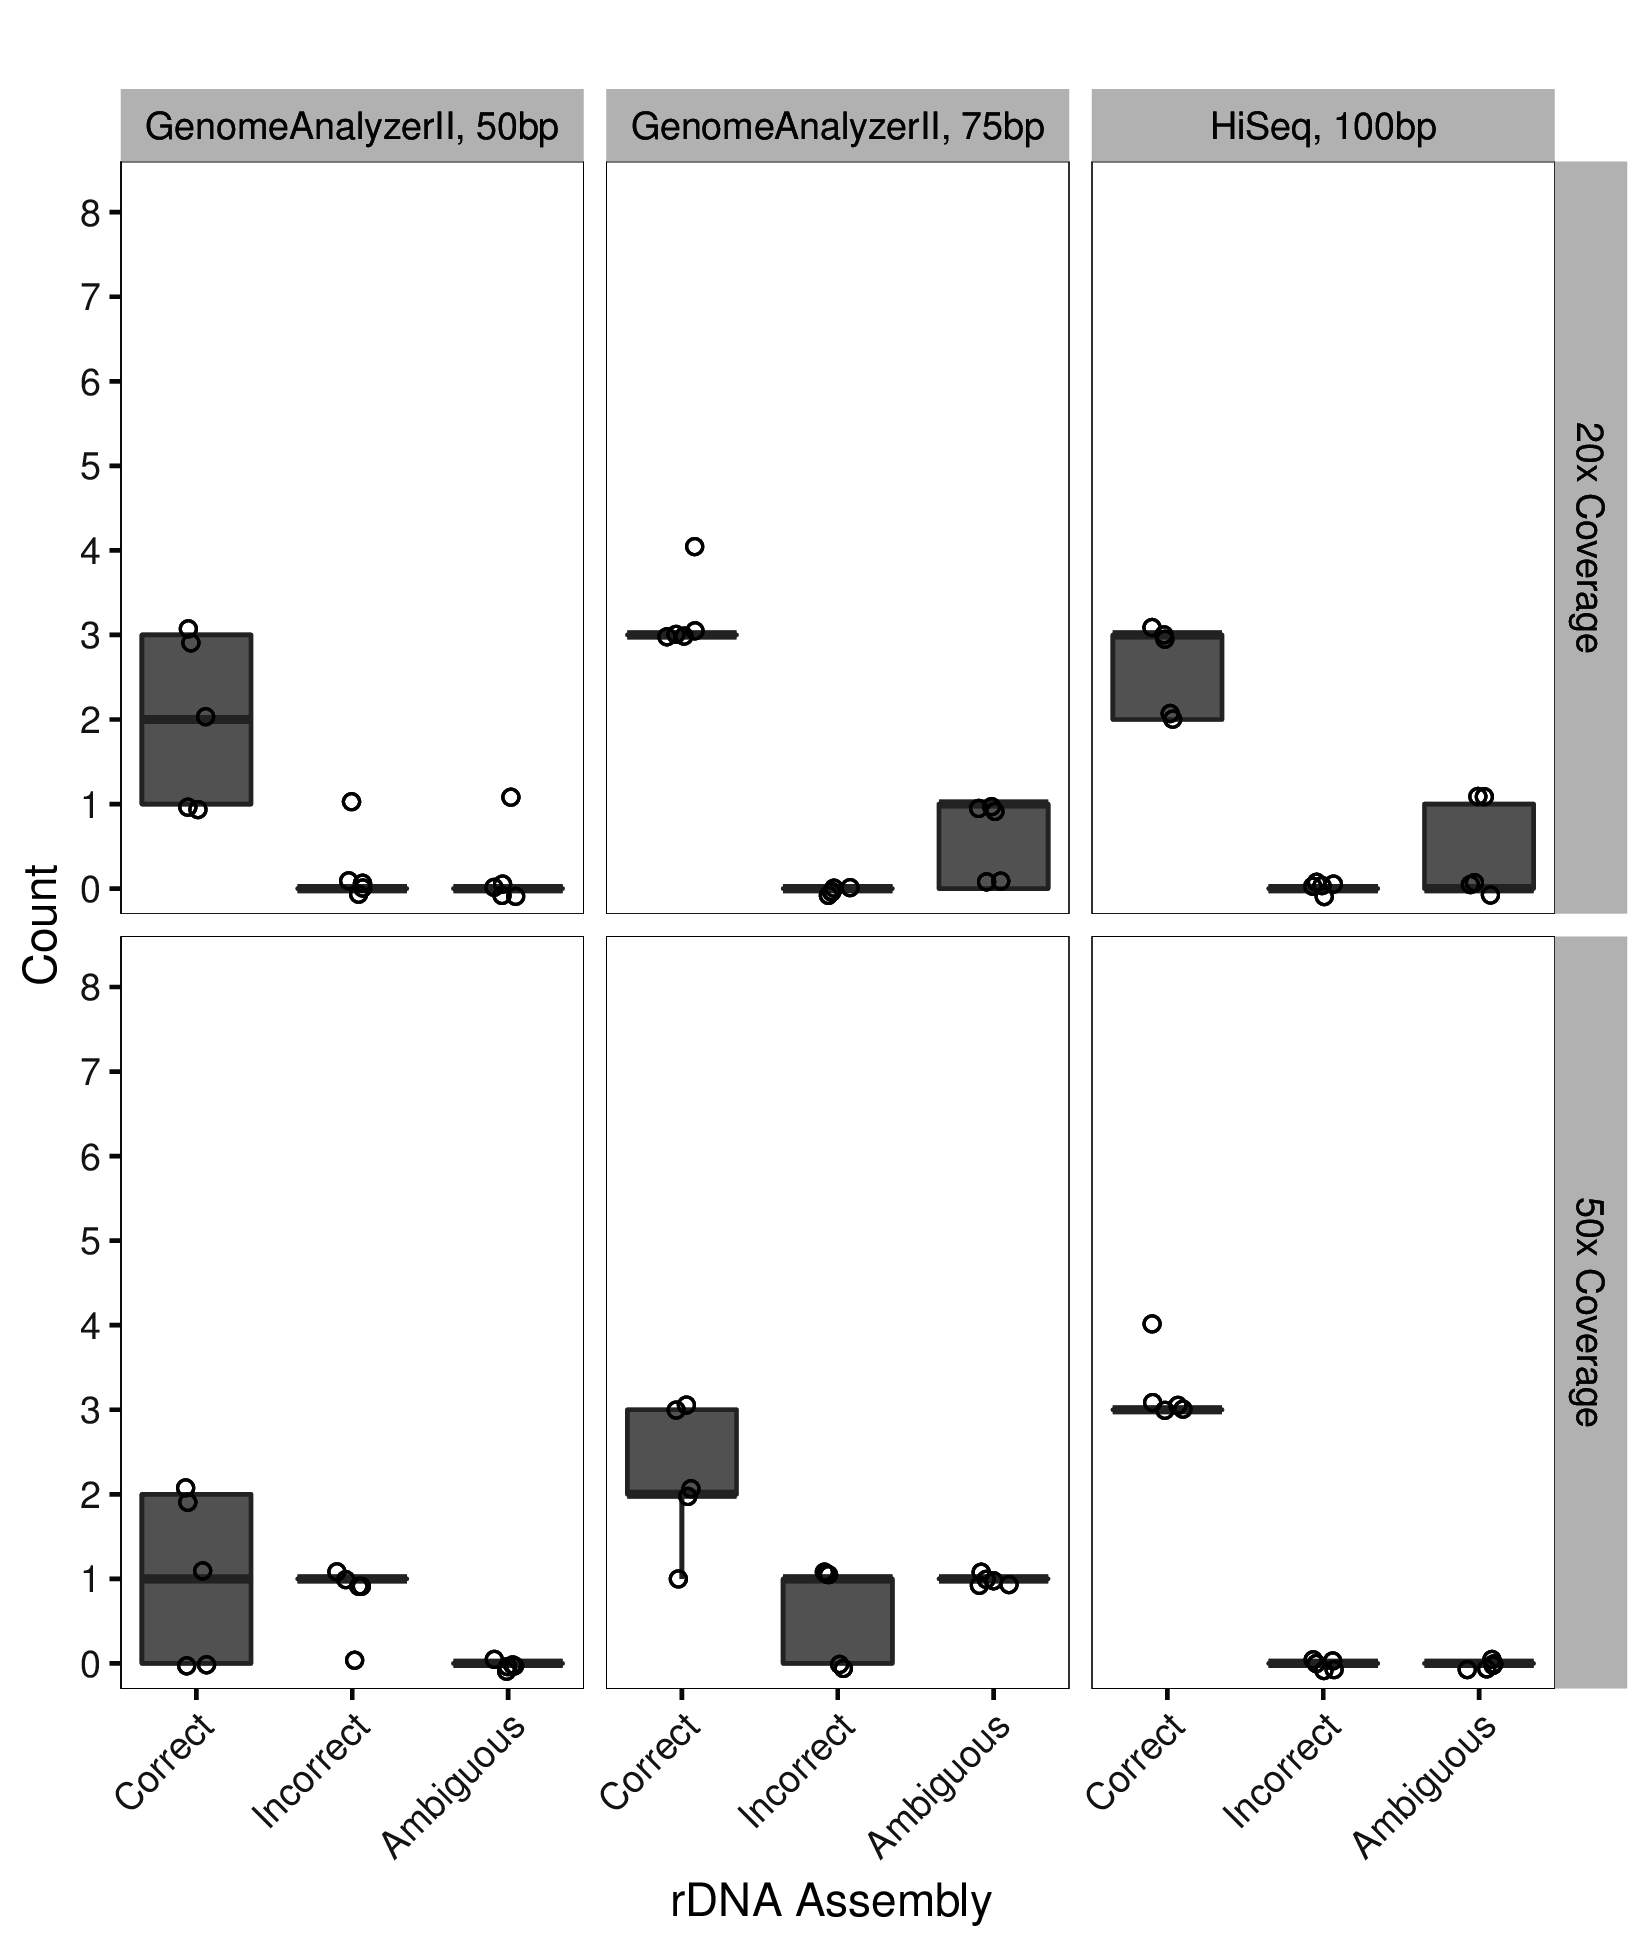
\includegraphics[width=.8\columnwidth]{kleb} %

    {\footnotesize \textbf{b.} \textit{K. pneumoniae} rDNA Assembly}
    \label{fig:sim_kleb}
  \end{minipage}%
  \caption{Comparison of \textit{de fere novo} assemblies of simulated reads generated by pIRS. In most cases, increasing coverage depth and read length resulted in fewer misassemblies. Assemblies were scored using \texttt{score}; the y axis reflects the total number of rDNAs in the genome (7 and 8 rDNAs, for \textit{E. coli} and \textit{K. pneumoniae} respectively). N=9.}
  \label{fig:simreads}
\end{figure}


\subsection*{Simulated reads with \textit{E. coli} and \textit{K. pneumoniae} genomes}

To investigate the effect of short read length on riboSeed assembly, pIRS\cite{Hu2012} was used to generate paired-end reads from the complete \textit{E. coli} MG1655 and \textit{K. pneumoniae} NTUH-K2044 genomes, simulating datasets at a range of read lengths most appropriate to the sequencing technology. In all cases, 300bp inserts with 10bp standard deviation and the built-in error profile were used. Coverage was simulated at 20x to emulate low coverage runs and at 50x to emulate coverage close to the optimized values determined by Miyamoto\cite{Miyamoto2014} and Desai\cite{Desai2013}. \textit{De fere novo} assembly was performed with riboSeed using \textit{E. coli} Sakai and \textit{K. pneumoniae} HS11286 as references, respectively, and the results were scored with \texttt{Score} (Figure \ref{fig:simreads}).


At either 20x or 50x coverage, \textit{de novo} assembly was unable to resolve any rDNAs with any of the simulated read sets. \textit{de fere novo} assembly with riboSeed showed modest improvement to both the \textit{E. coli} and \textit{K. pneumoniae} assemblies. Increasing depth of coverage and read length improves rDNA assemblies.




\subsection*{Benchmarking against hybrid sequencing and assembly}

To establish whether riboSeed performs as well with short reads obtained by sequencing a complete prokaryotic chromosome as with simulated reads, we attempted to assemble short reads from a published hybrid Illumina/PacBio sequencing project. The hybrid assembly using long reads was able to resolve rDNAs directly, and provides a benchmark against which to assess riboSeed performance in terms of: (i) bridging sequence correctly across rDNAs, and (ii) assembling rDNA sequence accurately within each cluster.


Sanjar, et al. published the genome sequence of \textit{Pseudomonas aeruginosa} BAMCPA07-48 (CP015377.1)\cite{Sanjar2016}, assembled from two libraries: ca. 270bp fragmented genomic DNA with 100bp paired-end reads sequenced on an Illumina HiSeq 4000 (SRR3500543), and long reads from PacBio RS II. The authors obtained a closed genome sequence by hybrid assembly. We ran the riboSeed pipeline on only the HiSeq dataset in order to compare \textit{de fere novo} assembly to the hybrid assembly and \textit{de novo} assembly of the same reads, using the related genome \textit{P. aeruginosa} ATCC 15692 (NZ\_CP017149.1) as a reference.

\textit{de fere novo} assembly correctly assembled across all 4 rDNA regions, whereas \textit{de novo} assembly failed to assemble any rDNA regions (Table \ref{table:assemblyresults}A).

Comparing the BAMCPA07-48 reference to the \textit{de fere novo} assembly, we found a total of 9 SNPs in the rDNA flanking regions (Table \ref{table:snps}). The same regions from the ATCC 15692 reference used in the \textit{de fere novo} assembly showed 108 SNPs compared to the BAMCPA07-48.  This demonstrates that this subassembly scheme successfuly recovers the correct sequence with remarkably few SNPs, despite a large number of differences between the reference and the sequenced isolate.

Further, to assess how riboSeed's assembly would compare to simply supplying the whole reference as a trusted contig to SPAdes (which, it is worth noting, is not recommended by the SPAdes authors), we assembled the same reads with the \textit{P. aeruginosa} ATCC 15692 as a trusted contig, and compared the results to the \textit{de fere novo} and \textit{de novo} assemblies. While \textit{de novo} assembly yielded the lowest error rates, and \textit{reference-based}  assembly yielded the longest contigs, \textit{de fere novo} assembly proved to be an optimal compromise, as it exhibited very low error rates, the highest genome recovery fraction, and the lowest number of contigs (Table S5).


Thus, we find that the \textit{de fere novo} assembly using short reads performs better than \textit{de novo} assembly using short reads alone. Comparison of the \textit{de fere novo} assembly to the hybrid assembly allows assessment of \textit{de fere novo} accuracy, and indicates that \textit{de fere novo} can recover the rDNA sequence correctly placed in their genomic context, and with a low error rate.

\begin{table}[!h]
\centering
\caption{rDNA region SNPs between hybrid assembly of \textit{P. aeruginosa} BAMCPA07-48 and \textit{de fere novo} assembly in rDNA regions, including 1kb upstream and downstream of the rDNA}
\label{table:snps}
\begin{tabular}{lcc}
  \toprule
  rDNA region & CP015377.1  & Substitution    \\
  (5S,16S,23S with flanking region) & Location &     \\
  \colrule
  \multirow{4}{*}{398001--405418}  & 402331     & T $\to$ C \\
              & 402332     & C $\to$ T \\
              & 404332     & C $\to$ T \\
              & 404380     & G $\to$ T \\
  \colrule
  1039539--1045687 &  ---          &  ---   \\
  \colrule
  \multirow{3}{*}{1862045--1869194} & 1864462    & A $\to$ G \\
              & 1868402    & A $\to$ C \\
              & 1868426    & A $\to$ T \\
  \colrule
  \multirow{2}{*}{2809154--2816303} & 2811180    & G $\to$ A \\
              & 2813886    & T $\to$ C \\
  \botrule
\end{tabular}
\end{table}



\subsection*{Case Study: Closing the assembly of \textit{S. aureus} UAMS-1}

% \begin{table*}[!t]
% \centering
%   \caption{Assembly of the \textit{S. aureus} UAMS-1}
%   \label{table:U1}
%   \begin{tabular}{p{5.2cm}p{.95cm}p{.75cm}p{.75cm}p{2.63cm}p{.6cm}>{\hfill}p{.4cm}p{.2cm}p{.1cm}>{\hfill}p{.4cm}p{.2cm}p{.1cm}}
%     % \arrayrulecolor{black}
%     \toprule
%     \multirow{2}{*}{Sequenced Strain Name} & \multirow{2}{*}{Platform}  & \multirow{2}{*}{Length} & \multirow{2}{*}{Depth}  &  \multicolumn{2}{c}{Reference Strain} &  \multicolumn{3}{c}{\textit{de novo}} & \multicolumn{3}{c}{\textit{de fere novo}} \\
%                             &   &   &   & Name & rDNAs  &  \textbf{$\checkmark$} & -- & $\times$ &  \textbf{\textbf{$\checkmark$}} & -- & $\times$  \\
%                             % \cmidrule{1-1}\cmidrule(l){2-2}\cmidrule(l){3-3}\cmidrule(l){4-4}\cmidrule(l){5-6}\cmidrule(l){7-9}\cmidrule(l){10-12}
%     \colrule
%     \textit{S.aureus} UAMS-1 & MiSeq & 300 & 110x & MRSA252  & 5 &  \textbf{0} & 5 & 0   & \textbf{2} & 3 & 0 \\
%     \botrule
%     \begin{minipage}[t]{.5\textwidth}
%       {\tiny
%         $\checkmark$ correct assembly; -- skipped assembly; $\times$ incorrect assembly
%       }
%     \end{minipage}
%   \end{tabular}
% \end{table*}

\textit{Staphylococcus aureus} UAMS-1 is a well-characterized, USA200 lineage, methicillin-sensitive strain isolated from an osteomyelitis patient. The corresponding published genome was sequenced using Illumina MiSeq generating 300bp reads, and the assembly refined with GapFiller as part of the BugBuilder pipeline \url{https://github.com/jamesabbott/BugBuilder}. Currently, the genome assembly is represented by two scaffolds (JTJK00000000), with several repeated regions acknowledged in the annotations\cite{Sassi2015}. As the rDNA regions were not fully characterized in the annotations, we proposed that \textit{de fere novo} assembly might resolve some of the problematic regions.

Using the same reference \textit{S. aureus} MRSA252\cite{Holden2004} (BX571856.1) with riboSeed as was used in the original assembly, \textit{de fere novo} assembly correctly bridged gaps corresponding to two of the five rDNAs in the reference genome (Table \ref{table:assemblyresults}B). Furthermore, \textit{de fere novo} assembly bridged two contigs that were syntenic with the ends of the scaffolds in the published assembly, indicating that the regions resolved by riboSeed could allow closure of the genome.


We modified the BugBuilder pipeline (\url{https://github.com/nickp60/BugBuilder}) used in the published assembly to incorporate pseudocontigs from riboSeed, resulting in a single scaffold of 7 contigs. In this case, riboSeed was able assist in bringing an existing high-quality scaffold to closure.


\subsection*{Benchmarking against GAGE-B Datasets}
% \begin{sidewaystable}
\begin{table*}[!hb]
  \centering
  \caption{Comparison of \textit{de novo} and riboSeed's \textit{de fere novo} assemblies}
  \label{table:assemblyresults}
  \begin{tabular}{p{.3cm}p{5.2cm}p{.95cm}p{.75cm}p{.75cm}p{2.63cm}p{.6cm}>{\hfill}p{.4cm}p{.2cm}p{.1cm}>{\hfill}p{.4cm}p{.2cm}p{.1cm}}
    % \arrayrulecolor{black}
    \toprule
    & \multirow{2}{*}{Sequenced Strain Name} & \multirow{2}{*}{Platform}  & \multirow{2}{*}{Length} & \multirow{2}{*}{Depth}  &  \multicolumn{2}{c}{Reference Strain} &  \multicolumn{3}{c}{\textit{de novo}} & \multicolumn{3}{c}{\textit{de fere novo}} \\
   & & & & & Name & rDNAs & \textbf{$\checkmark$} & -- & $\times$ & \textbf{$\checkmark$} & -- & $\times$  \\
   % \cmidrule{1-1}\cmidrule(l){2-2}\cmidrule(l){3-3}\cmidrule(l){4-4}\cmidrule(l){5-6}\cmidrule(l){7-9}\cmidrule(l){10-12}
    \toprule
   \textbf{A.}  & \textit{P. aeruginosa} BAMCPA07-48 & HiSeq & 100 & 200x & ATCC 15692  & 4 & \textbf{0} & 4 & 0 & \textbf{4} & 0 & 0 \\
    \botrule
   \textbf{B.} & \textit{S.aureus} UAMS-1 & MiSeq & 300 & 110x & MRSA252  & 5 &  \textbf{0} & 5 & 0   & \textbf{2} & 3 & 0 \\
    \toprule
    & \textit{A. hydrophila} SSU   & HiSeq   & 101   & 250   & ATCC 7966 & 10 & \textbf{0} & 10 & 0  & \textbf{4} & 6 & 0  \\

    % & \textit{B. cereus} VD118    & HiSeq   & 101   & 300  & ATCC 10987  & 12 & \textbf{0} & 12 & 0  & \textbf{1} & 11 & 0  \\

    & \textit{B. cereus} ATCC 10987   & MiSeq   & 250   & 100  & NC7401 & 14 & \textbf{0} & 14 & 0  & \textbf{12} & 2 & 0  \\

    & \textit{B. fragilis} HMW 615   & HiSeq   & 101   & 250   & 638R & 6 & \textbf{0} & 5 & 1  & \textbf{0} & 3 & 3  \\

    \textbf{C.} & \textit{R. sphaeroides} 2.4.1 & HiSeq & 101 & 210 & ATCC 17029  & 4 & \textbf{0} & 4 & 0  & \textbf{1} & 3 & 0  \\

    & \textit{R. sphaeroides} 2.4.1 & MiSeq & 251 & 100 & ATCC 17029  & 4 & \textbf{1} & 2 & 1  & \textbf{1} & 2 & 1  \\

    & \textit{S. aureus} M0927 & HiSeq & 101 & 250 & USA300\_TCH1516 & 5 & \textbf{0} & 5 & 0  & \textbf{3} & 2 & 0  \\

    & \textit{V. cholerae} CO 0132(5) & HiSeq & 100 & 110 & El Tor str. N16961  & 8 & \textbf{0} & 8 & 0  & \textbf{5} & 3 & 0  \\

    & \textit{V. cholerae} CO 0132(5) & MiSeq   & 250   & 100   & El Tor str. N16961 & 8 & \textbf{0} & 8 & 0  & \textbf{4} & 4 & 0  \\

    & \textit{X. axonopodis} pv. \textit{Manihotis} UA323 & HiSeq   & 101   & 250   & pv. \textit{Citrumelo} & 2 & \textbf{0} & 1 & 1  & \textbf{2} & 0 & 0 \\
    % \arrayrulecolor{black}

    \botrule
    \begin{minipage}[t]{.5\textwidth}
      {\tiny
        $\checkmark$  correct assembly; --  unnassembled; $\times$  incorrect assembly\\
        % * run with \texttt{--centers 7:0} option to group tandem rDNAs
      }
    \end{minipage}
  \end{tabular}
\end{table*}
% \end{sidewaystable}




We used the Genome Assembly Gold-standard Evaluation for Bacteria (GAGE-B) datasets \cite{Magoc2013} to assess the performance of riboSeed against a set of well-characterized assemblies. These datasets represent a broad range of challenges; low GC content and tandem rDNA repeats prove challenging to the riboSeed procedure.

\textit{Mycobacterium abscessus} has only a single rDNA operon and does not suffer from the issue of rDNA repeats, so it was excluded from this analysis.  Also excluded was the \textit{B. cereus} VD118 HiSeq dataset, as metagenomic analysis revealed likely contamination (see Figure S5 and ``Excluding GAGE-B HiSeq \textit{B. cereus}'' section in supplementary data).

When the reference used in the GAGE-B study came from the sequenced strain (as was the case for \textit{Rhodobacter sphaeroides}  and  \textit{Bacillus cereus}), we chose an alternate reference, as using the true reference sequence would provide an unfair advantage to riboSeed. The GAGE-B datasets include both raw and trimmed reads; in all cases, the trimmed reads were used. Results are shown in Table \ref{table:assemblyresults}C.

Compared to the \textit{de novo} assembly, \textit{de fere novo} assembly improved the majority of assemblies. In the case of the \textit{S. aureus} and \textit{R. sphaeroides} datasets, particular difficulty was encountered for all of the references tested. In the case of \textit{Bacteroides fragilis}, the entropy plot (Figure S4g) shows that the variability on the 5' end of the operon is much lower than the other strains, likely leading to the misassemblies.

\section*{DISCUSSION}
We demonstrate that the regions flanking equivalent rDNAs from related strains show a high degree of conservation in related organisms. This allows us to correctly place rDNAs within a newly sequenced isolate, even in the absence of the resolution that would be provided by long read sequencing. Comparing the regions flanking rDNAs within a single genome, we observed that when considering sufficiently large flanking regions, flanking sequences show enough variability to differentiate each instance of the rDNAs. Taken together with the cross-taxon homology, this allows inference of the location (i.e. the flanking regions) of rDNAs, and the variability of these flanking regions within a genome enables unique identification of reads likely belonging to each cluster.

The extent of sequence similarity between the sequenced isolate and the reference influences the resulting \textit{de fere novo} assembly. To prevent spurious joining of contigs, if fewer than 80\% of the reads map to the reference, the resulting pseudocontigs will be treated as ``untrusted'' contigs by SPAdes. Figure \ref{fig:degen} shows that although one should use the closest complete reference available for optimal results, the subassembly method is robust against moderate discrepancies between the reference and sequenced isolate's flanking regions.

The method of constructing pseudocontigs implemented by riboSeed relies on having a relevant reference sequence, where the rDNA regions act as ``bait'', fishing for reads that likely map specifically to that region. Although we show this to be an effective way to partition the appropriate reads, perhaps a more robust and supervision-free method would be to use a probabilistic representation of equivalent rDNA regions for a particular taxon. By developing a database of sequence profiles (e.g. hidden Markov Models) from each of the homologous rDNAs in a taxon, perhaps the step of choosing a single most appropriate reference could be circumvented. For datasets where the choice of reference determines riboSeed's effectiveness, a probabilistic approach may improve performance.

Several checks are implemented after the subassembly to ensure that the resulting pseudocontig is fit for inclusion in the next round in the next mapping/subassembly iteration or the final \textit{de fere novo} assembly. If a subassembly's longest contig is greater than 3x the particular pseudocontig length or shorter than 6kb (a conservative minimum length of a 16S, 23S, and 5S operon), this is taken to be a sign of poor parameter choice so the user is warned, and by default no further seedings will occur to avoid spurious assembly. Such an outcome can be indicative of any of several factors: improper clustering of operons; insufficient or extraneous flanking sequence; sub-optimal mapping; inappropriate choice of \textit{k}-mer length for subassembly; inappropriate reference; or other issues. If this occurs, we recommend testing the assembly with different \textit{k}-mers, changing the flanking length, or trying alternative reference genomes. Mapping depth of the rDNA regions is also reported for each iteration; a marked decrease in mapping depth may also be indicative of problems.

Many published genome finishing tools and approaches offer improvements when applied to suitable datasets, but none (including the approach presented in this paper) is able in isolation to resolve all bacterial genome assembly issues. One constraint on the performance of riboSeed is the quality of rRNA annotations in reference strains. Although it is impossible to concretely confirm it is the case \textit{in silico}, we (and others \cite{Mariano2016}) have found several reference genomes during the course of this study that we suspect have collapsed rDNA repeats. We recommend using a tool such as 16Stimator\cite{Perisin2016} or rrnDB\cite{Stoddard2014} to estimate number of 16S (and therefore rDNAs) prior to assembly, or riboStack to assess mapping depths after running riboSeed.

As riboSeed relies on de Bruijn graph assembly, the results can be affected by assembler parameters. Care should be taken to find the most appropriate settings, particularly in regard to read trimming approach, range of \textit{k}-mers, and error correction schemes.

One difficulty in determining the accuracy of rDNA counts in reference genome occures because genome sequences are often released without publishing the reads used to produce the genome assembly. This practice is a major hindrance when attempting to perform coverage-based quality assessment, such as to infer the likelihood of collapsed rDNAs. While data transparency is expected for gene expression studies, that stance has not been universally adopted when publishing whole-genome sequencing results. To ensure the highest quality assemblies, it is imperative that researchers allow the scientific community to scrutinize the raw whole genome sequencing data with the same rigor that would be applied to any other type of high-throughput sequencing project.




\section*{CONCLUSION}
Demonstration that rDNA flanking regions are conserved across taxa and that flanking regions of sufficient length are distinct within a genome allowed for the development of riboSeed, a \textit{de fere novo} assembly method. riboSeed  utilizes rDNA flanking regions to act as barcodes for repeated rDNAs, allowing the assembler to correctly place and orient the rDNA. \textit{de fere novo} assembly can improve the assembly by bridging across ribosomal regions, and, in cases where rDNA repeats would otherwise result in incomplete scaffolding, can result in closure of a draft genome when used in conjunction with existing polishing tools. Although riboSeed is far from a silver bullet to provide perfect assemblies from short read technology, it shows the utility of using genomic reference data and mixed assembly approaches to overcome algorithmic obstacles. This approach to resolving rDNA repeats may allow further insight to be gained from large public repositories of short read sequencing data, such as SRA, and when used in conjunction with other genome finishing techniques, provides an avenue towards genome closure.

\section{FUNDING}
The work was supported by a joint studentship between The James Hutton Institute, Dundee, Scotland, and the National University of Ireland, Galway, Ireland.


\section{ACKNOWLEDGEMENTS}
We thank Anton Korobeynikov for his recommendations on optimizing SPAdes. Yoann Augagneur, Shaun Brinsmade, and Mohamed Sassi graciously provided access to the \textit{S. aureus} UAMS-1 genome sequencing data.  Additional computational resources were provided by CLIMB\cite{Connor2016}. We thank the Bioconda\cite{Dale2017} community for their support.


\subsection{Conflict of interest statement.}
None declared.

\bibliographystyle{unsrt}
\bibliography{/home/nicholas/GitHub/riboSeed/Waters_et_al_2017/ms/riboSeed_refs}

\end{document}
